\section{Niveau 2}

Dans le niveau 2, les usines peuvent avoir plusieurs ressources d'entrée mais une ressource de sortie. Cependant, deux usines distinctes ne peuvent avoir la même ressource d'entrée. 

\subsection{Problématique introduite par l'extension du niveau 2}

Avec cette nouvelle définition, on aura besoin d'un graphe. Ce dernier remplacera notre structure \textit{chain} qui était composée d'une liste de liste d'usines. Nous faisons ce choix afin de faciliter la lecture des chaînes de production.\\
\indent Sur ce graphe, les noeuds représentent les usines, les arcs sortants représentent la production et les entrants la consommation.\\
\smallbreak
\indent Considérons l'exemple suivant : 
\begin{itemize}
    \item Usine1 consomme "Pain" et  "Lait" et produit "Pain perdu"
    \item Usine2 consomme "Orange" et Sucre" et produit "Jus"
    \item Usine3 consomme "Pain perdu" et "Jus" et produit "Dej"
\end{itemize}

\indent Ainsi, la chaîne de production est construite de la manière suivante :

\begin{figure}[H]
		\centering
		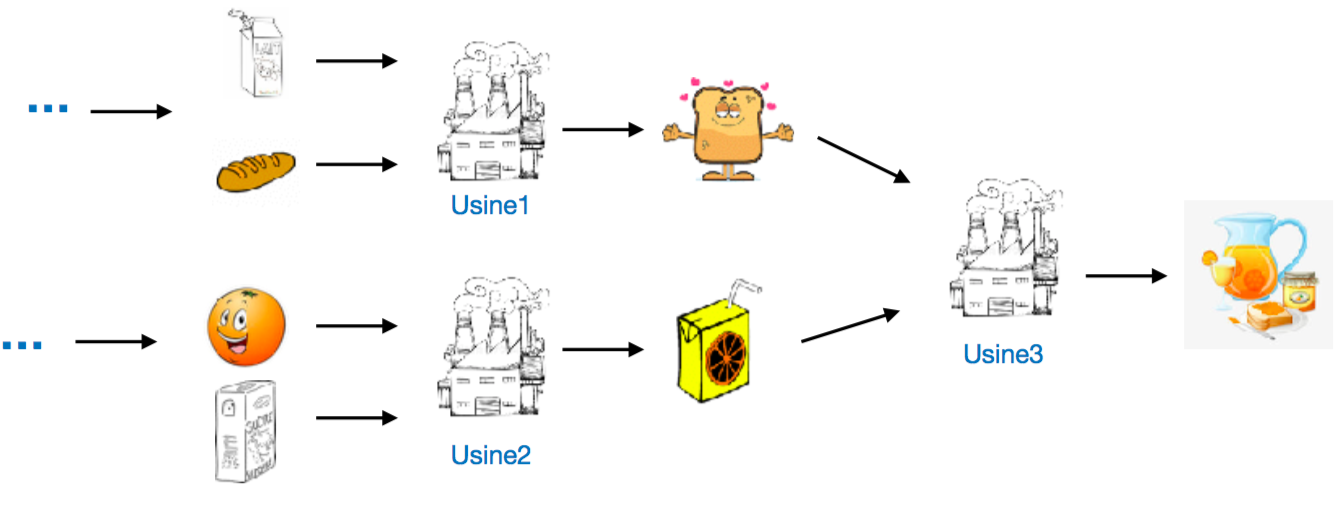
\includegraphics[scale=0.35]{factory_niveau2.png}
    	\caption{Exemple : représentation de la chaîne de production }
    \end{figure}

\indent Nous voyons bien à travers cette exemple que l'utilisation d'un graphe facilite la construction et la lecture de la chaîne de production.

\subsection{L'implémentation }

Nos structures \textit{factory, bench, chain} ne changent pas de forme vu qu'on a pas utilisé type racket et donc le langage n'est pas typé. Cependant, dans la structure \textit{factory}
qui est de la forme suivante,
\begin{verbatim} 
    (struct factory (consommation production cout))
\end{verbatim}
 le paramètre consommation n'est plus une paire mais une liste de paires au vu de la nouvelle définition de l'usine.\\ 
 \smallbreak
 De plus nous avons créé quatre nouvelles structures pour pouvoir créer le graphe :
\begin{verbatim}
    (struct graphe (node_racine lstnode lst-adj))
\end{verbatim}

Avec \textit{node\_racine} est le noeud racine, \textit{lstnode} une liste de noeud et \textit{lst-adj} une liste de liste d'entiers qui représente la liste des adjacences.

\begin{verbatim}
    (struct node (id factory))
\end{verbatim}

Avec \textit{id} un entier unique par noeud et \textit{factory} une structure factory.

\begin{verbatim}
    (struct arc (cout id-deb id-end))
\end{verbatim}


Avec \textit{cout id-deb id-deb} trois entiers :
$id-deb \xrightarrow{\text{cout}} id-end$


\begin{verbatim}
    (struct chemin (lst-id cout gain))
\end{verbatim}

Avec \textit{lst-id} la liste des id des noeud qui compose le chemin, \textit{cout} le prix d'achat du chemin et \textit{gain} la quantité de gold produite par le chemin.

Nous avons ici toutes les structures qui nous permettent d'implémenter un graphe. Nous allons donc maintenant étendre les algorithmes permettant de déterminer la quantité optimale de Gold produite en n tours. 

\subsection{Production du Gold optimale en n tours de jeu}

Pour produire une quantité de Gold optimale nous allons procéder de la même manière qu'au niveau 1. Nous allons analyser tous les chemins possibles pour ensuite choisir le meilleur. \\
\indent Ainsi par exemple, considérons le graphe de la figure 1.


\begin{figure}[H]
		\centering
		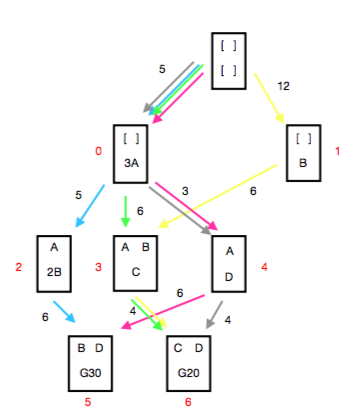
\includegraphics[scale=0.75]{graphee.png}
    	\caption{Exemple : Graphe de niveau 2 }
    \end{figure}
    
Ce graphe admet pour liste d'adjacence la liste suivante :

\begin{verbatim}
    {{2 3 4} {3} {5} {6} {5 6} {} {}}
\end{verbatim}

Avec 0 1 2 3 4 5 6 l'\textit{id} des noeuds.
(Le coût des noeuds 5 et 6 sont respectivement 6 et 4.

\indent Ainsi, la fonction \textit{best-road-tree}
détermine le meilleur chemin de l'arbre.
\indent Dans l'exemple ci-dessus :
\begin{itemize}
    \item Pour acheter l'usine 5 on doit emprunter le chemin bleu et rose. On sera donc amené à acheter les usines 0, 2, 4, 5. Finalement cette chaîne produira 5 Golds.
    \item Pour acheter l'usine 6 on peut emprunter différents chemins:
    \begin{itemize}
        \item Le chemin jaune et gris. Cette chaîne sera en déficit de 34 Golds.
        \item Le chemin vert et gris. Cette chaîne sera en déficit de 2 Golds.
    \end{itemize}

\end{itemize}

Nous pouvons donc en conclure que le meilleur chemin est le rose. 

\subsection{Les différentes stratégies}

Dans cette sous-partie nous allons proposer des stratégies de rendement efficace. Malheureusement, nous ne les avons pas toutes implémentées, par faute de temps.

\subsubsection{Random}

La stratégie \textit{Random} consiste à choisir une chaîne d'usines au hasard sous réserve qu'elle produise du Gold. \\
\indent Ainsi par exemple, sur la figure 3 nous pouvons choisir soit le chemin bleu et rose qui nous permet l'achat de l'usine 5, soit les chemins vert et gris ou jaune et gris pour acheter l'usine 6. \\
\indent Elle ne choisira pas par exemple le chemin bleu et gris car ces chemins ne permettent ni l'achat de l'usine 5 ni celui de l'usine 6.

\subsubsection{Toujours la moins chère}

La stratégie \textit{Toujours la moins chère} consiste à choisir les usines moins chères. Si nous reprenons la figure 6, notre algorithme choisirai d'abord l'usine 0 ($5 < 12$) puis l'usine 4 ($3 < 5 <6)$ et enfin l'usine 5 qui crée du Gold. Le premier chemin choisi est donc le rose puis on sera contraint de choisir le chemin bleu pour pouvoir acheter l'usine 5.

\subsubsection{Usine à plus forte production de Gold}

La stratégie \textit{Usine à plus forte production de Gold} consiste à choisir l'usine qui produit le plus de Gold et ensuite choisit les chemins nécessaires pour arriver à cette usine. Par exemple, si l'usine 6 produisait 40 Golds et non 20, l'algorithme choisirait à fortiori le chemin gris et le chemin jaune ou vert au hasard.

\subsubsection{Meilleur rendement}
 
La stratégie \textit{Meilleur rendement} achète les usines qui permettent un meilleur rendement. Nous avons vu le fonctionnement de l'algorithme dans la partie 3.3.\\
\smallbreak

\subsection{L'extension du niveau trois}

A ce stade du projet, les usines peuvent avoir plusieurs ressources d'entrée et de sortie. Nous n'avons pas eu le temps de l'implémenter. Néanmoins, si nous n'étions pas restreint par le temps nous aurions choisi comme pour le niveau 2 un graphe. Cependant, il aurait été un peu plus complexe car plusieurs arcs peuvent sortir d'un seul et même noeud. 
 